\documentclass[uplatex,dvipdfmx]{jsarticle}

\usepackage{amsmath}
\usepackage{bm}
\usepackage{float}
\usepackage{graphicx}
\usepackage{xcolor}
\usepackage{listings}

\lstset{
language=Python,
frame=single,
backgroundcolor=\color{gray!10},
basicstyle=\ttfamily\small,
keywordstyle=\color{blue}\bfseries,
commentstyle=\color{green!50!black},
stringstyle=\color{red},
numbers=left,
numberstyle=\tiny,
breaklines=true
}

\title{シミュレーション理工学 レポートその1}
\author{%
特別聴講学生（東京学芸大学）\\
情報理工学域\\
26A2001 樋田巧
}
\date{提出日 2026年6月12日}

\begin{document}

\maketitle

\section{演習1 問題2}

\subsection{課題}
オイラーリチャードソン法を用い、惑星の回転運動をシミュレーションするプログラムを作成する。作成したプログラムを用いて、時間刻みによる最大の回転半径の変化を調べよ（時間刻みは2 桁程度変化させて調べること）。

\subsection{計算原理と用いた式}

太陽を原点に固定し，惑星の運動のみを考える。万有引力の法則とニュートンの運動方程式より，惑星の運動は

\begin{equation}
\frac{d^2x}{dt^2}
=
-\frac{GM}{r^3}x
\end{equation}

\begin{equation}
\frac{d^2y}{dt^2}
=
-\frac{GM}{r^3}y
\end{equation}

で表される。ただし，

\begin{equation}
r=\sqrt{x^2+y^2}
\end{equation}

である。

今回の授業では，長さを 1 AU，時間を 1 年で規格化している。このとき，

\begin{equation}
GM = 4\pi^2
\end{equation}

となるため，プログラムではこの値を用いた。

また，2階微分方程式を1階連立微分方程式に変換すると，

\begin{equation}
\frac{dx}{dt}=v_x
\end{equation}

\begin{equation}
\frac{dy}{dt}=v_y
\end{equation}

\begin{equation}
\frac{dv_x}{dt}
=
-\frac{GM}{r^3}x
\end{equation}

\begin{equation}
\frac{dv_y}{dt}
=
-\frac{GM}{r^3}y
\end{equation}

となる。これらの式をオイラー・リチャードソン法によって数値的に解いた。

\subsection{プログラムの考え方}

初期条件として，

\[
x=1,\quad y=0
\]

\[
v_x=0,\quad v_y=2\pi
\]

を与えた。

まず現在位置から加速度を求め，その値を用いて時間刻みの半分だけ進めた中間点の位置と速度を計算する。その後，中間点での加速度を求め，その値を用いて位置と速度を更新した。

時間刻み $\Delta t$ は 0.001 から 0.100 まで変化させ，各条件についてシミュレーションを行った。計算中に半径

\[
r=\sqrt{x^2+y^2}
\]

を毎ステップ計算し，その最大値を $r_{\max}$ として記録した。

得られた $\Delta t$ と $r_{\max}$ の関係を出力し，gnuplot を用いてグラフ化した。

\subsection{実行結果と考察}

図\ref{fig:rmax}に時間刻み $\Delta t$ と最大回転半径 $r_{\max}$ の関係を示す。

\begin{figure}[H]
	\centering
	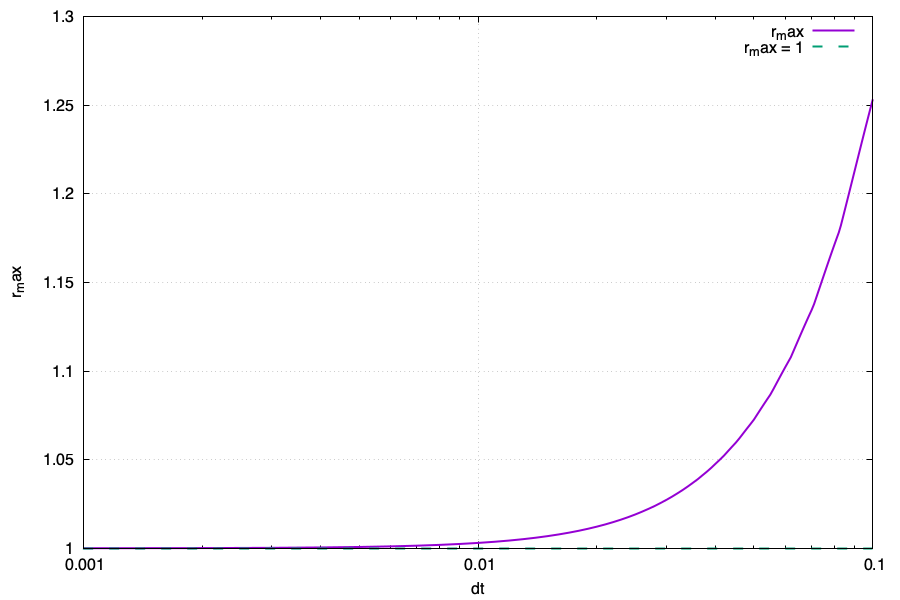
\includegraphics[width=0.8\textwidth]{./figures/r_max.png}
	\caption{時間刻み $\Delta t$ と最大回転半径 $r_{\max}$ の関係}
	\label{fig:rmax}
\end{figure}

図より，時間刻みが大きい場合は $r_{\max}$ が 1 から大きくずれていることが分かる。一方で，時間刻みを小さくするにつれて $r_{\max}$ は 1 に近づいている。

理想的な円軌道では半径は常に 1 AU であるため，最大回転半径も 1 となるはずである。しかし，数値計算では時間を離散的に扱うため，時間刻みが大きいと近似誤差が大きくなり，軌道が理想的な円軌道からずれてしまう。その結果，最大回転半径も大きくなったと考えられる。

今回の結果から，オイラー・リチャードソン法では時間刻みを小さくすることで計算精度が向上し，理論値に近い結果が得られることを確認できた。


\section{演習2 問題3}

\subsection{課題}
講義資料「2重星」の問題に対するシミュレーションを行い，「軌道の分類」に対応する結果を求めよ。注：この結果は惑星軌道の判定法に依存するので，必ずしも全く同じ結果が得られるとは限らない。

\subsection{計算原理と用いた式}

座標平面上に2つの恒星を固定し，その位置を

\[
(-1,0), \quad (1,0)
\]

とした。

質点は2つの恒星から重力を受けるため，それぞれの恒星との距離を

\[
r_1=\sqrt{(x+1)^2+y^2}
\]

\[
r_2=\sqrt{(x-1)^2+y^2}
\]

とすると，加速度は

\begin{equation}
\frac{dv_x}{dt}
=
-\frac{x+1}{r_1^3}
-\frac{x-1}{r_2^3}
\end{equation}

\begin{equation}
\frac{dv_y}{dt}
=
-\frac{y}{r_1^3}
-\frac{y}{r_2^3}
\end{equation}

で表される。

また，位置と速度の関係は

\begin{equation}
\frac{dx}{dt}=v_x
\end{equation}

\begin{equation}
\frac{dy}{dt}=v_y
\end{equation}

である。

これらの連立1階微分方程式をオイラー・リチャードソン法によって数値的に解いた。

\subsection{プログラムの考え方}

質点の初期位置は

\[
x=0.1,\quad y=1.0
\]

とした。

また，初速度の向きや大きさを変化させて計算を行った。

各時刻において現在位置から加速度を求め，その値を用いて時間刻みの半分だけ進めた中間点の位置と速度を計算した。その後，中間点での加速度を求め，その値を用いて位置と速度を更新した。

時間刻みは

\[
\Delta t = 0.001
\]

とし，

\[
t = 10
\]

まで計算を行った。

初速度の向きや大きさを複数変更して計算を行い，その中から軌道の特徴が分かりやすい結果を選択した。

\subsection{実行結果と考察}

本シミュレーションでは，初速度の向きとして水平方向，鉛直方向，斜め方向の3種類を設定し，さらにそれぞれについて速度成分の大きさを12通り変化させた。したがって，合計36通りの初期条件について計算を行った。

その結果，多くの条件では質点が二重星系から遠ざかり，閉じた軌道を形成せずに発散する様子が見られた。一方で，いくつかの条件では特徴的な軌道が確認できたため，その代表例を図\ref{fig:vertical}〜図\ref{fig:diagonal}に示す。

\begin{figure}[H]
\centering
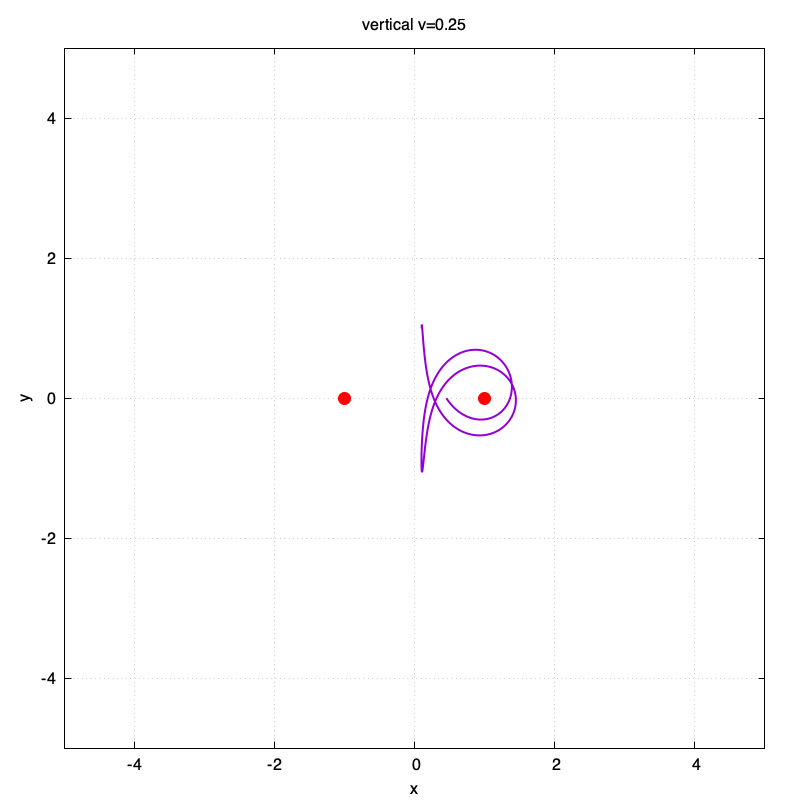
\includegraphics[width=0.7\textwidth]{./figures/orbit_vertical_0.png}
\caption{鉛直方向の初速度を与えた場合}
\label{fig:vertical}
\end{figure}

図\ref{fig:vertical}では，質点は右側の恒星の周囲を回るような軌道を描いていることが分かる。

\begin{figure}[H]
\centering
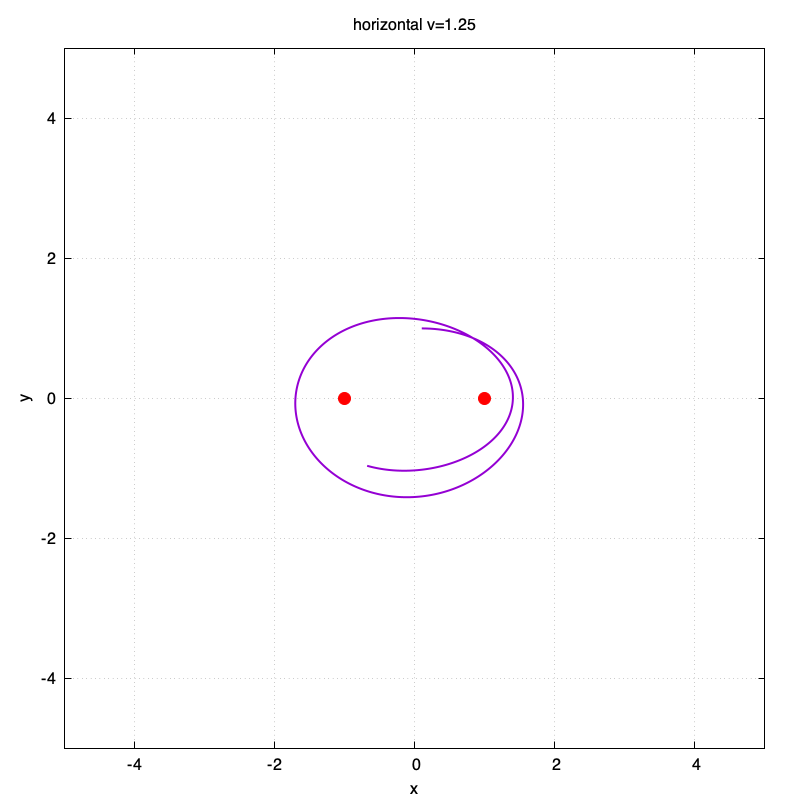
\includegraphics[width=0.7\textwidth]{./figures/orbit_horizontal_4.png}
\caption{水平方向の初速度を与えた場合}
\label{fig:horizontal}
\end{figure}

図\ref{fig:horizontal}では，質点は2つの恒星をまとめて囲むような軌道を描いている。

\begin{figure}[H]
\centering
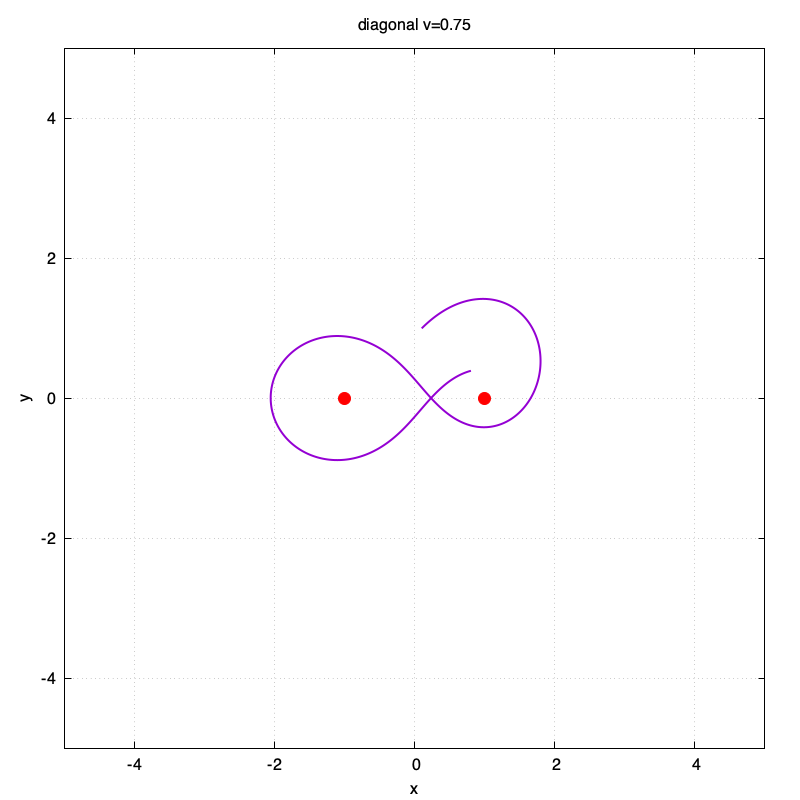
\includegraphics[width=0.7\textwidth]{./figures/orbit_diagonal_2.png}
\caption{斜め方向の初速度を与えた場合}
\label{fig:diagonal}
\end{figure}

図\ref{fig:diagonal}では，質点が2つの恒星の間を通過しながら運動し，8の字のような軌道を描いていることが確認できる。

今回のシミュレーションでは，初速度の向きや速度成分の設定を変えることで軌道の形が大きく変化した。多くの場合は質点が系外へ飛び出してしまったが，一部の条件では恒星の重力によって束縛され，特徴的な軌道を形成した。

鉛直方向に初速度を与えた場合は一方の恒星の周囲を回る軌道となり，水平方向に初速度を与えた場合は2つの恒星を囲む軌道となった。また，斜め方向に初速度を与えた場合には，両方の恒星の近くを通過する8の字状の軌道が確認できた。

このことから，二重星系における質点運動では初期条件によって軌道の性質が大きく変化することが分かった。また，同じ重力場であっても，一方の恒星を周回する軌道，二重星全体を周回する軌道，両恒星の間を通過する軌道など，多様な運動が現れることを確認できた。

\section{演習3 問題3}

\subsection{課題}

適応的時間幅アルゴリズムを用いて，講義資料「三体問題」の問題の中から問題を2つ選択してシミュレーションを行い，適応的時間幅アルゴリズムの効果を調査せよ。

\subsection{計算原理と用いた式}

電子1，電子2の位置をそれぞれ

\[
\bm{r}_1=(x_1,y_1)
\]

\[
\bm{r}_2=(x_2,y_2)
\]

とする。

このとき，電子1，電子2の運動方程式は

\begin{equation}
\frac{d^2\bm{r}_1}{dt^2}
=
-2\frac{\bm{r}_1}{|\bm{r}_1|^3}
+
\frac{\bm{r}_1-\bm{r}_2}{|\bm{r}_1-\bm{r}_2|^3}
\end{equation}

\begin{equation}
\frac{d^2\bm{r}_2}{dt^2}
=
-2\frac{\bm{r}_2}{|\bm{r}_2|^3}
-
\frac{\bm{r}_1-\bm{r}_2}{|\bm{r}_1-\bm{r}_2|^3}
\end{equation}

で表される。

本課題では，これらの式をオイラー・リチャードソン法によって数値的に解いた。

\subsection{プログラムの考え方}

初期条件として，初期条件Aでは

\[
\bm{r}_1=(2.0,0), \quad \bm{r}_2=(-1.0,0)
\]

\[
\bm{v}_1=(0,0.95), \quad \bm{v}_2=(0,-1)
\]

を与えた。

また，初期条件Bでは

\[
\bm{r}_1=(1.4,0), \quad \bm{r}_2=(-1.0,0)
\]

\[
\bm{v}_1=(0,0.86), \quad \bm{v}_2=(0,-1)
\]

を与えた。

運動方程式は演習1と同様にオイラー・リチャードソン法によって数値的に解いた。

固定時間幅法では，

\[
\Delta t = 0.001
\]

を一定として計算を行った。

一方，適応時間幅法では，同じ時間区間を

\[
dt
\]

で1回計算した結果と，

\[
\frac{dt}{2}
\]

で2回計算した結果を比較し，その差を局所誤差の指標とした。

誤差が設定値より大きい場合には時間幅を半分にし，十分小さい場合には時間幅を2倍にすることで，計算中に時間幅を自動的に調整した。

計算時間は

\[
t=80
\]

までとし，各時刻における電子の位置，エネルギー，および初期エネルギーとの差である energy\_error を出力した。

その後，固定時間幅法と適応時間幅法について，電子軌道および energy\_error の比較を行った。

\subsection{実行結果と考察}

図\ref{fig:problem1_orbit}に初期条件Aにおける軌道を示す。

\begin{figure}[H]
	\centering
	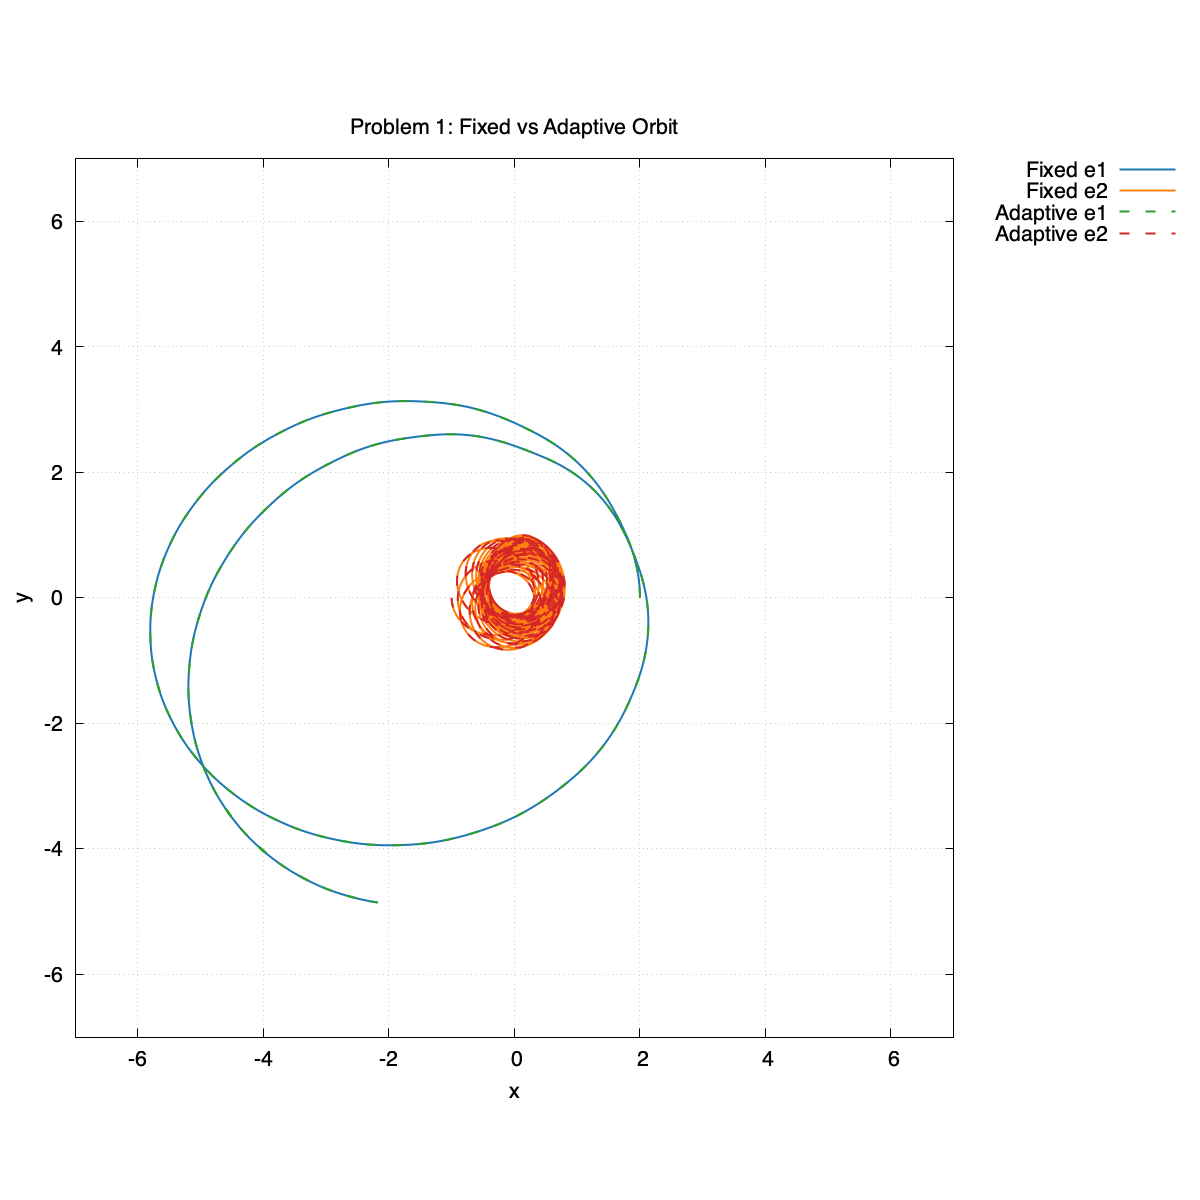
\includegraphics[width=0.75\textwidth]{./figures/problem1_orbit_compare.png}
	\caption{初期条件Aにおける軌道の比較}
	\label{fig:problem1_orbit}
\end{figure}

初期条件Aでは，固定時間幅と適応時間幅で軌道の始点および電子の運動の大まかな特徴は共通しているものの，長時間計算では軌道は完全には一致していないことが分かる。特に電子2の軌道では，固定時間幅と適応時間幅で軌道半径や軌跡に違いが見られた。一方で，どちらの場合も電子1は大きな軌道を描き，電子2は原点付近を周回していることから，運動の大まかな特徴は保たれていると考えられる。

図\ref{fig:problem2_orbit}に初期条件Bにおける軌道を示す。

\begin{figure}[H]
	\centering
	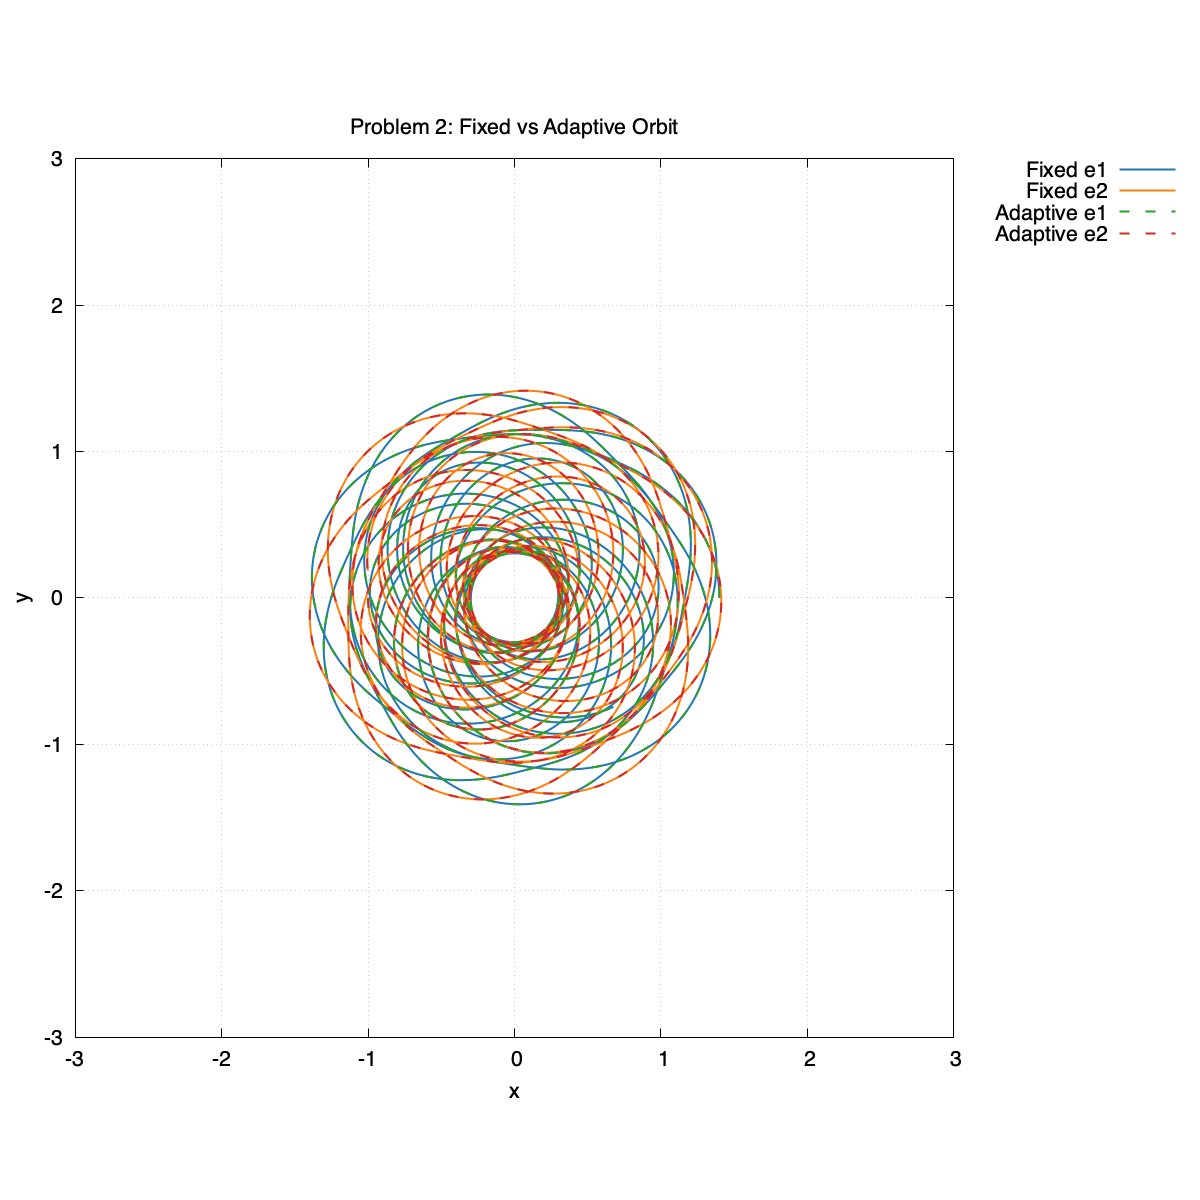
\includegraphics[width=0.75\textwidth]{./figures/problem2_orbit_compare.png}
	\caption{初期条件Bにおける軌道の比較}
	\label{fig:problem2_orbit}
\end{figure}

初期条件Bでは，固定時間幅と適応時間幅の軌道はほぼ重なっており，大きな違いは見られなかった。したがって，この条件では時間幅の制御方法による軌道への影響は比較的小さいと考えられる。

次に，初期エネルギーとの差である energy\_error を比較した。

図\ref{fig:problem1_energy}に初期条件Aにおける energy\_error を示す。

\begin{figure}[H]
	\centering
	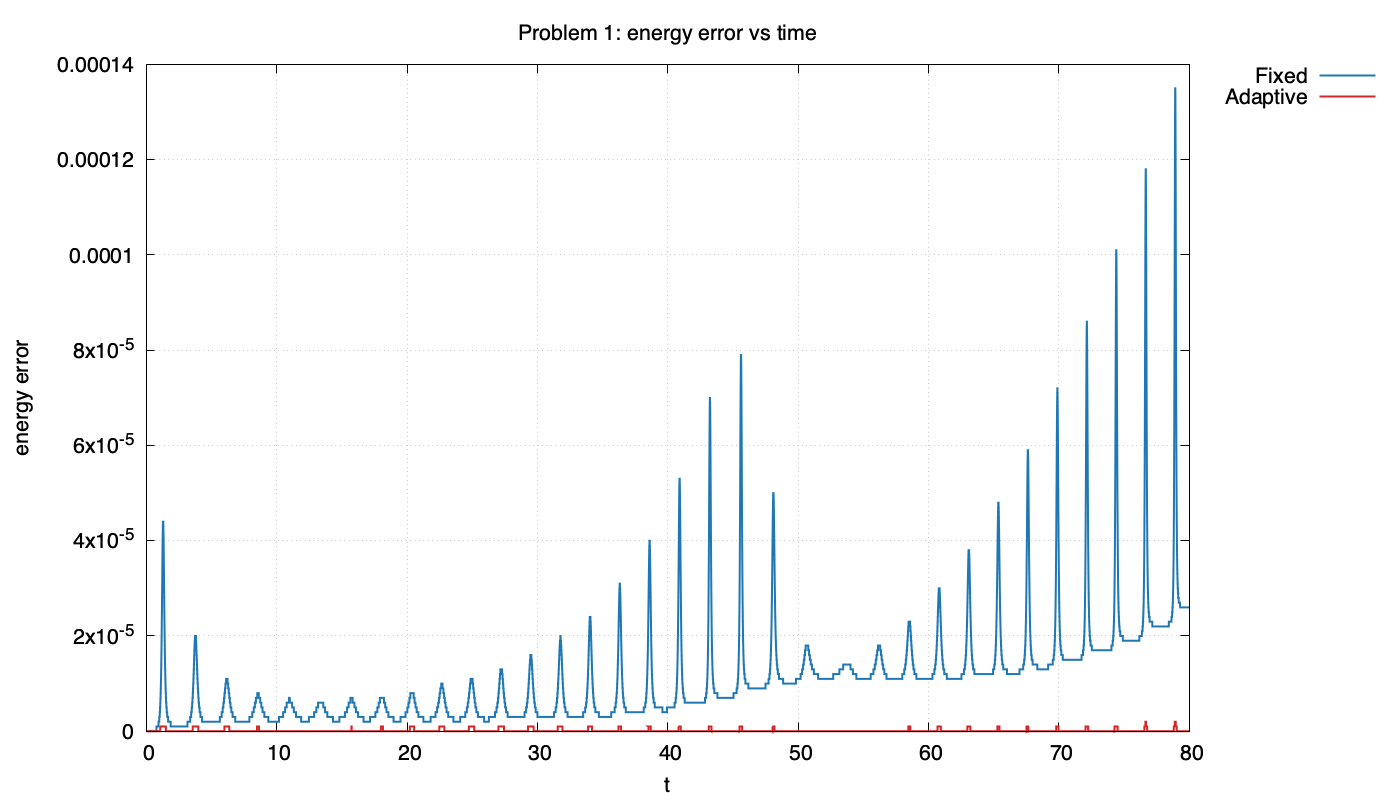
\includegraphics[width=0.75\textwidth]{./figures/problem1_energy_error.png}
	\caption{初期条件Aにおける energy\_error の比較}
	\label{fig:problem1_energy}
\end{figure}

固定時間幅では energy\_error が時間とともに増加しており，周期的に大きなピークが現れていることが分かる。一方，適応時間幅では energy\_error が全体を通して非常に小さく抑えられている。

初期条件Aでは，固定時間幅の最大 energy\_error は

\[
1.35\times10^{-4}
\]

であった。一方，適応時間幅の最大 energy\_error は

\[
2.0\times10^{-6}
\]

であり，誤差が大幅に減少していることが確認できた。

図\ref{fig:problem2_energy}に初期条件Bにおける energy\_error を示す。

\begin{figure}[H]
	\centering
	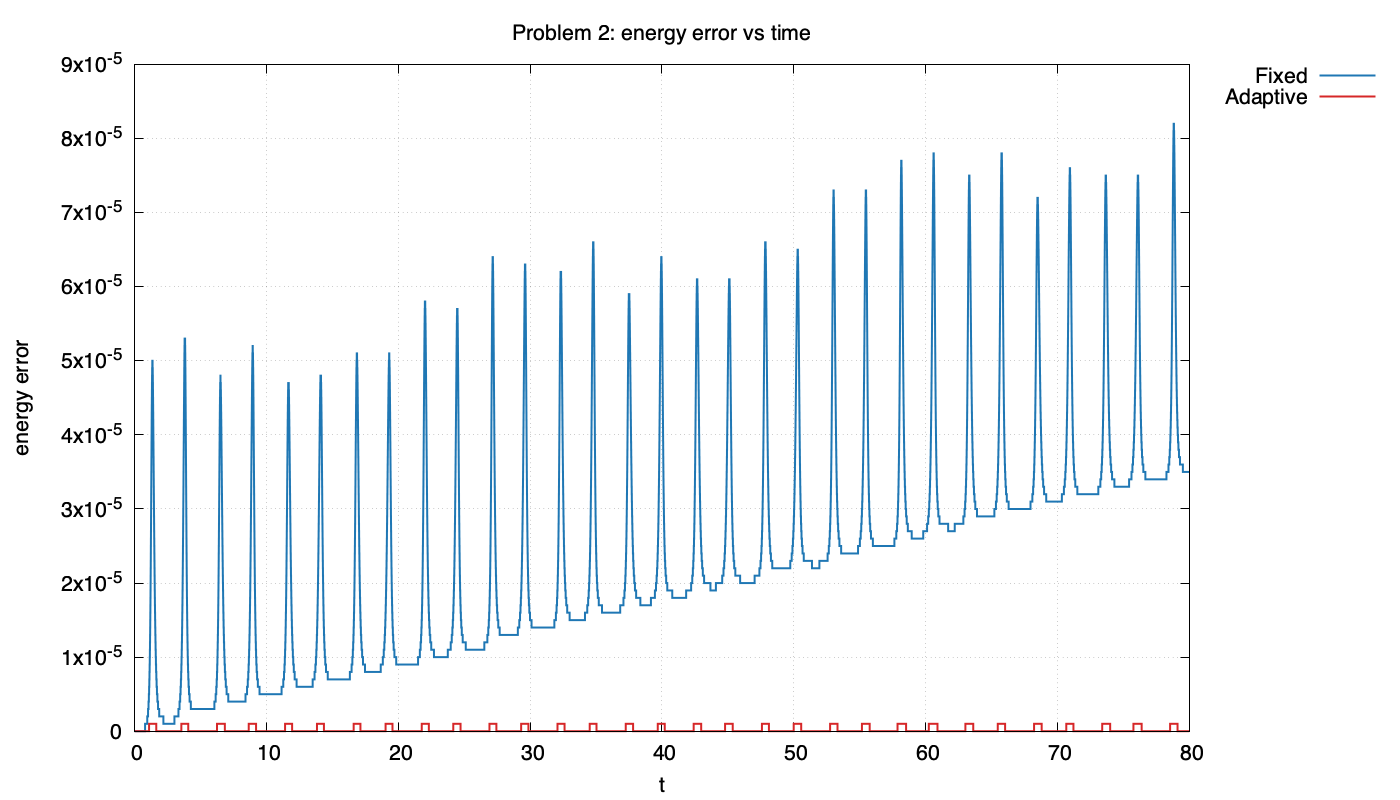
\includegraphics[width=0.75\textwidth]{./figures/problem2_energy_error.png}
	\caption{初期条件Bにおける energy\_error の比較}
	\label{fig:problem2_energy}
\end{figure}

初期条件Bにおいても，固定時間幅では energy\_error が徐々に増加している。一方，適応時間幅では energy\_error が非常に小さく保たれている。

初期条件Bでは，固定時間幅の最大 energy\_error は

\[
8.2\times10^{-5}
\]

であった。一方，適応時間幅の最大 energy\_error は

\[
1.0\times10^{-6}
\]

であり，こちらも固定時間幅より小さい値となった。

以上の結果より，初期条件A，初期条件Bのどちらについても，今回用いた固定時間幅 $dt=0.001$ と比較して，適応時間幅を用いた場合の方が energy\_error を大幅に減少させることができた。特に初期条件Aでは軌道そのものにも違いが見られたことから，長時間計算では誤差の蓄積が軌道へ影響を与えることが分かる。

一方，適応時間幅では運動の変化が大きい部分で時間幅を小さくし，変化が小さい部分で時間幅を大きくすることで，計算精度を保ちながら誤差の増大を抑えることができた。

このことから，適応時間幅アルゴリズムは今回の電子軌道計算条件において有効であり，固定時間幅 $dt=0.001$ の場合よりも高い精度でシミュレーションを行えたことが確認できた。

\section{プログラム}

\subsection{演習1 問題2}

\begin{lstlisting}
#include <stdio.h>
#include <stdlib.h>
#include <math.h>

#define GM (4.0 * M_PI * M_PI)

double eulerRichardson(const double dt);

int main(void) {
	FILE *radius_fp = fopen("r_max_data.txt", "w");

	if (radius_fp == NULL) {
		return 1;
	}

	for (int i = 100; i >= 1; i--) {
		const double dt = i * 0.001;
		const double r_max = eulerRichardson(dt);
		fprintf(radius_fp, "%f %f\n", dt, r_max);
	}

	fclose(radius_fp);
	return 0;
}

double eulerRichardson(const double dt) {
	const double t_max = 1.0;
	const int max = (int)(t_max / dt);

	double x = 1.0;
	double y = 0.0;
	double vx = 0.0;
	double vy = 2.0 * M_PI;
	double r_max = 0.0;

	for (int i = 0; i < max; i++) {
		const double r = sqrt(x * x + y * y);

		if (r > r_max) {
			r_max = r;
		}

		const double r3 = r * r * r;
		const double ax = -GM * x / r3;
		const double ay = -GM * y / r3;

		const double x_mid = x + 0.5 * vx * dt;
		const double y_mid = y + 0.5 * vy * dt;
		const double vx_mid = vx + 0.5 * ax * dt;
		const double vy_mid = vy + 0.5 * ay * dt;

		const double r_mid = sqrt(x_mid * x_mid + y_mid * y_mid);
		const double r3_mid = r_mid * r_mid * r_mid;
		const double ax_mid = -GM * x_mid / r3_mid;
		const double ay_mid = -GM * y_mid / r3_mid;

		vx += ax_mid * dt;
		vy += ay_mid * dt;
		x += vx_mid * dt;
		y += vy_mid * dt;
	}

	return r_max;
}
\end{lstlisting}


\subsection{演習2 問題3}

\begin{lstlisting}
#include <stdio.h>
#include <stdlib.h>
#include <math.h>

#define GM (1.0)
#define STAR_DISTANCE (1.0)

enum State { X, Y, N };

void calcAcceleration(const double pos[N], double acc[N]);
void eulerRichardson(const char filename[], const double vx0, const double vy0);

int main(void) {
	const double v_list[] = {0.25, 0.5, 0.75, 1.0, 1.25, 1.5, 1.75, 2.0, 2.25, 2.5, 2.75, 3.0};
	const int v_num = 12;

	for (int i = 0; i < v_num; i++) {
		char filename[100];

		sprintf(filename, "orbit_horizontal_%d.dat", i);
		eulerRichardson(filename, v_list[i], 0.0);

		sprintf(filename, "orbit_vertical_%d.dat", i);
		eulerRichardson(filename, 0.0, v_list[i]);

		sprintf(filename, "orbit_diagonal_%d.dat", i);
		eulerRichardson(filename, v_list[i], v_list[i]);
	}

	return 0;
}

void calcAcceleration(const double pos[N], double acc[N]) {
	const double star1[N] = {-STAR_DISTANCE, 0.0};
	const double star2[N] = { STAR_DISTANCE, 0.0};

	acc[X] = 0.0;
	acc[Y] = 0.0;

	const double dx1 = star1[X] - pos[X];
	const double dy1 = star1[Y] - pos[Y];
	const double r1 = sqrt(dx1 * dx1 + dy1 * dy1);
	const double r13 = r1 * r1 * r1;

	acc[X] += GM * dx1 / r13;
	acc[Y] += GM * dy1 / r13;

	const double dx2 = star2[X] - pos[X];
	const double dy2 = star2[Y] - pos[Y];
	const double r2 = sqrt(dx2 * dx2 + dy2 * dy2);
	const double r23 = r2 * r2 * r2;

	acc[X] += GM * dx2 / r23;
	acc[Y] += GM * dy2 / r23;
}

void eulerRichardson(const char filename[], const double vx0, const double vy0) {
	FILE *fp = fopen(filename, "w");

	if (fp == NULL) {
		return;
	}

	const double dt = 0.001;
	const double t_max = 10.0;
	const int max = (int)(t_max / dt);

	double pos[N] = {0.1, 1.0};
	double vel[N] = {vx0, vy0};
	double acc[N] = {0.0, 0.0};

	for (int i = 0; i < max; i++) {
		calcAcceleration(pos, acc);

		const double pos_mid[N] = {
			pos[X] + 0.5 * vel[X] * dt,
			pos[Y] + 0.5 * vel[Y] * dt
		};

		const double vel_mid[N] = {
			vel[X] + 0.5 * acc[X] * dt,
			vel[Y] + 0.5 * acc[Y] * dt
		};

		double acc_mid[N] = {0.0, 0.0};
		calcAcceleration(pos_mid, acc_mid);

		vel[X] += acc_mid[X] * dt;
		vel[Y] += acc_mid[Y] * dt;

		pos[X] += vel_mid[X] * dt;
		pos[Y] += vel_mid[Y] * dt;

		fprintf(fp, "%f %f\n", pos[X], pos[Y]);
	}

	fclose(fp);
}
\end{lstlisting}


\subsection{演習3 問題3}

\begin{lstlisting}
#include <stdio.h>
#include <stdlib.h>
#include <math.h>

#define Z (2.0)
#define DT (0.001)
#define DT_MIN (0.000001)
#define DT_MAX (0.004)
#define T_MAX (80.0)
#define ERROR_LIMIT (0.00000001)
#define NE (2)

#define PROBLEM1 (1)
#define PROBLEM2 (2)

enum State { X, Y, N };
enum Electron { E1, E2 };

void setInitialCondition(
	const int problem,
	double pos[NE][N],
	double vel[NE][N]
);
void calcAcceleration(
	const double pos[NE][N],
	double acc[NE][N]
);
void eulerRichardsonStep(
	const double pos[NE][N],
	const double vel[NE][N],
	const double dt,
	double next_pos[NE][N],
	double next_vel[NE][N]
);
double calcEnergy(
	const double pos[NE][N],
	const double vel[NE][N]
);
double calcDifference(
	const double pos1[NE][N],
	const double pos2[NE][N],
	const double vel1[NE][N],
	const double vel2[NE][N]
);
void copyState(
	const double src_pos[NE][N],
	const double src_vel[NE][N],
	double dst_pos[NE][N],
	double dst_vel[NE][N]
);
void fixedStepSimulation(
	const char filename[],
	const int problem
);
void adaptiveStepSimulation(
	const char filename[],
	const int problem
);

int main(void) {
	fixedStepSimulation("problem1_fixed.dat", PROBLEM1);
	adaptiveStepSimulation("problem1_adaptive.dat", PROBLEM1);

	fixedStepSimulation("problem2_fixed.dat", PROBLEM2);
	adaptiveStepSimulation("problem2_adaptive.dat", PROBLEM2);

	return 0;
}

void setInitialCondition(
	const int problem,
	double pos[NE][N],
	double vel[NE][N]
) {
	if (problem == PROBLEM1) {
		pos[E1][X] = 2.0;
		pos[E1][Y] = 0.0;
		pos[E2][X] = -1.0;
		pos[E2][Y] = 0.0;

		vel[E1][X] = 0.0;
		vel[E1][Y] = 0.95;
		vel[E2][X] = 0.0;
		vel[E2][Y] = -1.0;
	} else {
		pos[E1][X] = 1.4;
		pos[E1][Y] = 0.0;
		pos[E2][X] = -1.0;
		pos[E2][Y] = 0.0;

		vel[E1][X] = 0.0;
		vel[E1][Y] = 0.86;
		vel[E2][X] = 0.0;
		vel[E2][Y] = -1.0;
	}
}

void calcAcceleration(
	const double pos[NE][N],
	double acc[NE][N]
) {
	const double r1 = sqrt(pos[E1][X] * pos[E1][X] + pos[E1][Y] * pos[E1][Y]);
	const double r2 = sqrt(pos[E2][X] * pos[E2][X] + pos[E2][Y] * pos[E2][Y]);
	const double dx = pos[E1][X] - pos[E2][X];
	const double dy = pos[E1][Y] - pos[E2][Y];
	const double r12 = sqrt(dx * dx + dy * dy);

	const double r13 = r1 * r1 * r1;
	const double r23 = r2 * r2 * r2;
	const double r123 = r12 * r12 * r12;

	acc[E1][X] = -Z * pos[E1][X] / r13 + dx / r123;
	acc[E1][Y] = -Z * pos[E1][Y] / r13 + dy / r123;

	acc[E2][X] = -Z * pos[E2][X] / r23 - dx / r123;
	acc[E2][Y] = -Z * pos[E2][Y] / r23 - dy / r123;
}

void eulerRichardsonStep(
	const double pos[NE][N],
	const double vel[NE][N],
	const double dt,
	double next_pos[NE][N],
	double next_vel[NE][N]
) {
	double acc[NE][N];
	double pos_mid[NE][N];
	double vel_mid[NE][N];
	double acc_mid[NE][N];

	calcAcceleration(pos, acc);

	for (int e = 0; e < NE; e++) {
		for (int k = 0; k < N; k++) {
			pos_mid[e][k] = pos[e][k] + 0.5 * vel[e][k] * dt;
			vel_mid[e][k] = vel[e][k] + 0.5 * acc[e][k] * dt;
		}
	}

	calcAcceleration(pos_mid, acc_mid);

	for (int e = 0; e < NE; e++) {
		for (int k = 0; k < N; k++) {
			next_vel[e][k] = vel[e][k] + acc_mid[e][k] * dt;
			next_pos[e][k] = pos[e][k] + vel_mid[e][k] * dt;
		}
	}
}

double calcEnergy(
	const double pos[NE][N],
	const double vel[NE][N]
) {
	double kinetic = 0.0;

	for (int e = 0; e < NE; e++) {
		kinetic += 0.5 * (
			vel[e][X] * vel[e][X] + vel[e][Y] * vel[e][Y]
		);
	}

	const double r1 = sqrt(pos[E1][X] * pos[E1][X] + pos[E1][Y] * pos[E1][Y]);
	const double r2 = sqrt(pos[E2][X] * pos[E2][X] + pos[E2][Y] * pos[E2][Y]);
	const double dx = pos[E1][X] - pos[E2][X];
	const double dy = pos[E1][Y] - pos[E2][Y];
	const double r12 = sqrt(dx * dx + dy * dy);

	return kinetic - Z / r1 - Z / r2 + 1.0 / r12;
}

double calcDifference(
	const double pos1[NE][N],
	const double pos2[NE][N],
	const double vel1[NE][N],
	const double vel2[NE][N]
) {
	double diff = 0.0;

	for (int e = 0; e < NE; e++) {
		for (int k = 0; k < N; k++) {
			diff += fabs(pos1[e][k] - pos2[e][k]);
			diff += fabs(vel1[e][k] - vel2[e][k]);
		}
	}

	return diff;
}

void copyState(
	const double src_pos[NE][N],
	const double src_vel[NE][N],
	double dst_pos[NE][N],
	double dst_vel[NE][N]
) {
	for (int e = 0; e < NE; e++) {
		for (int k = 0; k < N; k++) {
			dst_pos[e][k] = src_pos[e][k];
			dst_vel[e][k] = src_vel[e][k];
		}
	}
}

void fixedStepSimulation(
	const char filename[],
	const int problem
) {
	FILE *fp = fopen(filename, "w");

	if (fp == NULL) {
		printf("file open error: %s\n", filename);
		return;
	}

	double pos[NE][N];
	double vel[NE][N];
	double next_pos[NE][N];
	double next_vel[NE][N];

	setInitialCondition(problem, pos, vel);

	const double energy0 = calcEnergy(pos, vel);
	const int max = (int)(T_MAX / DT);

	for (int i = 0; i < max; i++) {
		const double t = i * DT;
		const double energy = calcEnergy(pos, vel);
		const double energy_error = fabs(energy - energy0);

		fprintf(
			fp,
			"%f %f %f %f %f %f %f %f\n",
			t,
			pos[E1][X], pos[E1][Y],
			pos[E2][X], pos[E2][Y],
			DT,
			energy,
			energy_error
		);

		eulerRichardsonStep(pos, vel, DT, next_pos, next_vel);
		copyState(next_pos, next_vel, pos, vel);
	}

	fclose(fp);
}

void adaptiveStepSimulation(
	const char filename[],
	const int problem
) {
	FILE *fp = fopen(filename, "w");

	if (fp == NULL) {
		printf("file open error: %s\n", filename);
		return;
	}

	double pos[NE][N];
	double vel[NE][N];
	double full_pos[NE][N];
	double full_vel[NE][N];
	double half_pos[NE][N];
	double half_vel[NE][N];
	double half2_pos[NE][N];
	double half2_vel[NE][N];

	setInitialCondition(problem, pos, vel);

	const double energy0 = calcEnergy(pos, vel);
	double t = 0.0;
	double dt = DT;

	fprintf(
		fp,
		"%f %f %f %f %f %f %f %f\n",
		t,
		pos[E1][X], pos[E1][Y],
		pos[E2][X], pos[E2][Y],
		dt,
		energy0,
		0.0
	);

	while (t < T_MAX) {
		if (t + dt > T_MAX) {
			dt = T_MAX - t;
		}

		eulerRichardsonStep(pos, vel, dt, full_pos, full_vel);

		eulerRichardsonStep(pos, vel, 0.5 * dt, half_pos, half_vel);
		eulerRichardsonStep(half_pos, half_vel, 0.5 * dt, half2_pos, half2_vel);

		const double error = calcDifference(full_pos, half2_pos, full_vel, half2_vel);

		if (error > ERROR_LIMIT && dt > DT_MIN) {
			dt *= 0.5;
			continue;
		}

		copyState(half2_pos, half2_vel, pos, vel);
		t += dt;

		const double energy = calcEnergy(pos, vel);
		const double energy_error = fabs(energy - energy0);

		fprintf(
			fp,
			"%f %f %f %f %f %f %f %f\n",
			t,
			pos[E1][X], pos[E1][Y],
			pos[E2][X], pos[E2][Y],
			dt,
			energy,
			energy_error
		);

		if (error < 0.25 * ERROR_LIMIT && dt < DT_MAX) {
			dt *= 2.0;
		}
	}

	fclose(fp);
}
\end{lstlisting}

\section{AI利用について}

本課題では，コードエディタとして Visual Studio Code を使用した。

Visual Studio Code には GitHub Copilot によるコード補完機能が標準で導入されており，コーディング中にサジェスチョンが表示される場合がある。本課題のプログラムは講義資料の内容に沿って自ら作成したが，コーディング時にはこれらの補完機能を利用した。

また，演習3 問題3では，適応的時間幅アルゴリズムを用いたシミュレーションを行った。

適応的時間幅アルゴリズムの動作や結果の解釈について理解が十分でなかったため，理解補助を目的として ChatGPT（OpenAI）を利用した。

AIはプログラムの実行や図の生成は行わず，講義内容の理解，実験結果の整理，および結果の解釈の補助として利用した。

実際には長時間にわたり複数回のやり取りを行ったため，以下に，実際に使用したプロンプトと回答を，さらにAIで要約したものを示す。

\subsection*{利用例1：適応的時間幅アルゴリズムの理解}

\paragraph{プロンプト}

\begin{quote}
演習で適応的時間幅アルゴリズムを使っています。

固定時間幅との違いがよく分かりません。

私にもわかるように説明して下さい。
\end{quote}

\paragraph{AIの回答（要約）}

\begin{quote}
固定時間幅では計算中ずっと同じ時間幅を用いる。

一方，適応時間幅では変化が大きい部分では時間幅を小さくし，変化が小さい部分では時間幅を大きくする。

そのため必要な部分だけ細かく計算できる。
\end{quote}

\subsection*{利用例2：結果図の解釈}

\paragraph{プロンプト}

\begin{quote}
（軌道図を添付）

こんな結果になりました。

これはあっていますか？
\end{quote}

\paragraph{AIの回答（要約）}

\begin{quote}
軌道図を見る限り，計算自体は正常に行われているように見える。

ただし，適応時間幅アルゴリズムの効果を確認するためには，まず時間幅 $dt$ が実際に変化しているか調べる必要がある。
\end{quote}

\subsection*{利用例3：時間幅の変化について質問}

\paragraph{プロンプト}

\begin{quote}
（dt と時間の関係を表すグラフを添付）

時間幅が変化していることは分かりました。

次は何を確認すればよいですか？
\end{quote}

\paragraph{AIの回答（要約）}

\begin{quote}
時間幅が一定ではなく変化していることは確認できる。

適応時間幅アルゴリズムの効果を評価するためには，固定時間幅の場合と energy\_error を比較するとよい。
\end{quote}

\subsection*{利用例4：説明が難しかったため追加で質問}

\paragraph{プロンプト}

\begin{quote}
いいですね。

今，私の理解を超えてしまっています。

私にもわかるように説明して下さい。
\end{quote}

\paragraph{AIの回答（要約）}

\begin{quote}
高速道路では周囲の変化が少ないため，大まかに様子を見ても問題ない。

一方，交差点付近では変化が大きいため，より細かく確認する必要がある。

適応時間幅アルゴリズムも同様に，変化が大きい部分では細かく計算し，変化が小さい部分では大きな時間幅で計算していると考えられる。
\end{quote}

\subsection*{利用例5：誤差の比較結果について質問}

\paragraph{プロンプト}

\begin{quote}
（energy\_error の比較図を添付）

固定時間幅と適応時間幅の energy\_error を比較したところ，

適応時間幅の方が小さくなりました。

この結果はどのように考察できますか？
\end{quote}

\paragraph{AIの回答（要約）}

\begin{quote}
適応時間幅では，変化の大きい部分で時間幅を小さくして計算するため，誤差が小さくなると考えられる。

今回の結果では，適応時間幅の方が energy\_error が小さくなっており，固定時間幅よりも精度よく計算できていることが分かる。
\end{quote}

\subsection*{利用例6：考察内容の確認}

\paragraph{プロンプト}

\begin{quote}
Problem1では最大誤差がかなり小さくなり，

Problem2でも同様に誤差が小さくなりました。

この結果からどのような考察ができますか？
\end{quote}

\paragraph{AIの回答（要約）}

\begin{quote}
問題1，問題2のどちらについても，適応時間幅を用いた場合は固定時間幅より energy\_error が小さくなった。

このことから，適応時間幅アルゴリズムを用いることで，計算誤差を小さくできることが確認できる。
\end{quote}

以上のように，AIは講義内容の理解補助および結果の解釈補助のために利用した。

\end{document}
